\documentclass{beamer}
\usepackage[utf8]{inputenc}

\usepackage{utopia} %font utopia imported
\usepackage{caption}
\usepackage{graphicx}
\usepackage{xcolor}
\captionsetup[figure]{labelformat=empty}% redefines the caption setup of the figures environment in the beamer class.
\usetheme{Dresden}
\usecolortheme{beaver}

%------------------------------------------------------------
%This block of code defines the information to appear in the
%Title page
\title[] %optional
{WikipediaSearch}

\subtitle{An application of Personalized PageRank on a Wikipedia subset}

\author
{Roberto Corti}

\institute{Information Retrieval exam}

\date
{\today}

\titlegraphic{
\includegraphics[width=4.2cm,keepaspectratio]{logo-universita.png}
	\hspace*{13.04mm}~
	
\includegraphics[width=3.5cm,keepaspectratio]{logo-dssc.png}
}




%End of title page configuration block
%------------------------------------------------------------



%------------------------------------------------------------
%The next block of commands puts the table of contents at the 
%beginning of each section and highlights the current section:

\AtBeginSection[]
{
	\begin{frame}
		\frametitle{Outline}
		\tableofcontents[currentsection]
	\end{frame}
}
%------------------------------------------------------------


\begin{document}
	
	%The next statement creates the title page.
	\frame{\titlepage}
	
	%---------------------------------------------------------
	%This block of code is for the table of contents after
	%the title page
	\begin{frame}
		\frametitle{Outline}
		\tableofcontents
	\end{frame}
	%---------------------------------------------------------
	
	\section{Introduction}
	
	\begin{frame}
		\frametitle{WikipediaSearch}
		\framesubtitle{\textit{A brief introduction}}
		\only<1>{
			\textbf{WikipediaSearch} is a user-interactive tool that computes a Personalized (or Topic Specific) PageRank over a Wikipedia corpus.
		}
		
		\only<2>{ 
			\begin{figure}
				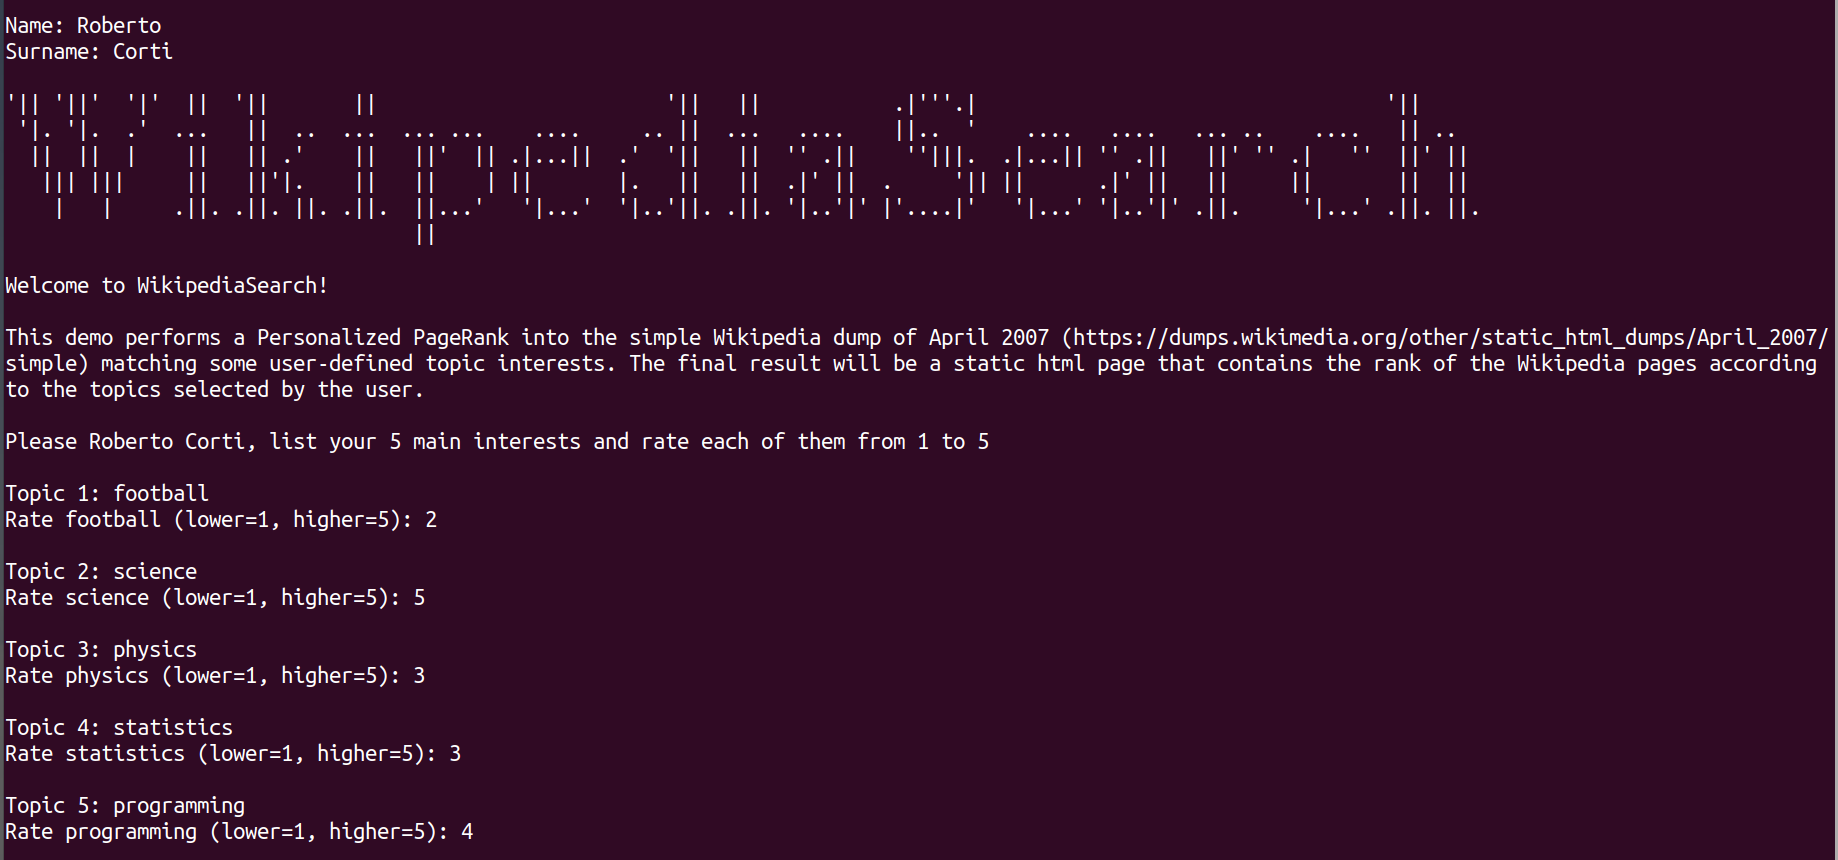
\includegraphics[scale=0.13]{input.png}
				\vspace{0.3cm}
				\caption{\textbf{Input interface}: user specifies the topics in which he/she has more interest} 
			\end{figure}  
				}
				
		\only<3>{ 
			\begin{figure}[t]
				
\includegraphics[scale=0.12]{output.png}
				\vspace{0.3cm}
				\caption{\textbf{Output page}: a rank of Wikipedia articles in which the user would be interested to read}
			\end{figure}  
		}
	
		
	\end{frame}
	
	\begin{frame}[t]
		\frametitle{The problem}
		\framesubtitle{\textit{"Bringing Order to the Web"}}
		\small{Algorithm developed by L. Page and S. Brin (Google co-founders) used to determine the order of web pages}\\
		
		\vspace{0.6cm}
		%\centering
		\textbf{Problem:} Is there a rating system that could measure the human interest and attention devoted to web pages? \\
		\vspace{0.5cm}
		\onslide<2->{
			\textbf{PageRank idea:} modeling the behavior of a "random surfer" in the Web graph.
		}
		
		
		
	\end{frame}

	\begin{frame}
		\frametitle{A recap of PageRank theory}
		\framesubtitle{\textit{From L.Page and S.Brin (1998)}}
		
		\only<1>{
			\begin{columns}
				\column{0.5\textwidth}
				\begin{figure}[t]
					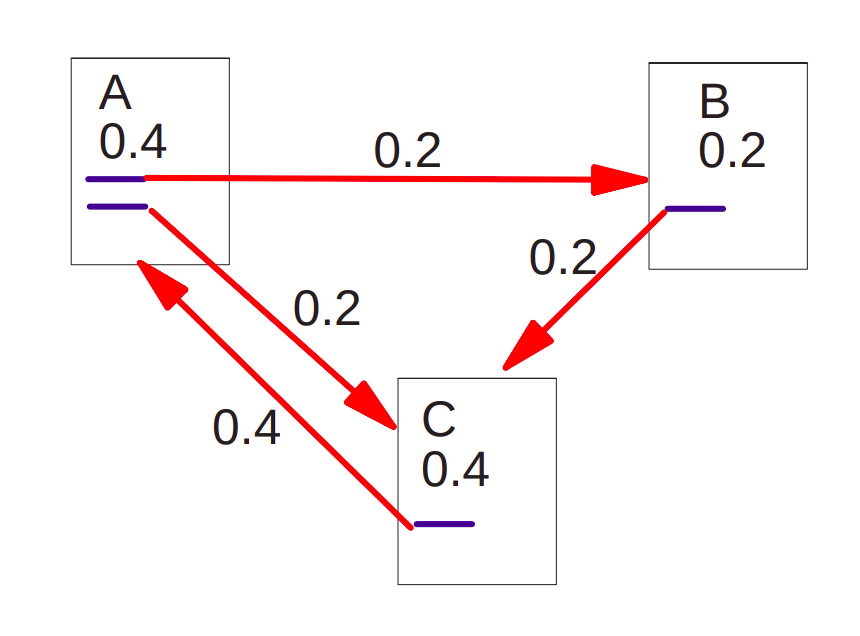
\includegraphics[scale=0.13]{webgraph.png}
				\end{figure}
				\column{0.65\textwidth}
				
				 $\vec{x}: $ probability distribution vector of the nodes\\
				\vspace{0.1cm} $M: $ square, stochastic matrix corresponding to the 
				directed grap where $M_{ij} = 1/N_j$\\
				\vspace{0.2cm}
				$\Rightarrow$ Find the stationary probability distribution $\Leftrightarrow$ find the unique stochastic eigenvector of to the eigenvalue 1: 
				$$ M\vec{\pi} = \vec{\pi} $$ 
				$\vec{\pi} = $ PageRank vector
			\end{columns} 
		}
		
		\only<2>{
			\begin{columns}
				\column{0.5\textwidth}
				\begin{figure}
					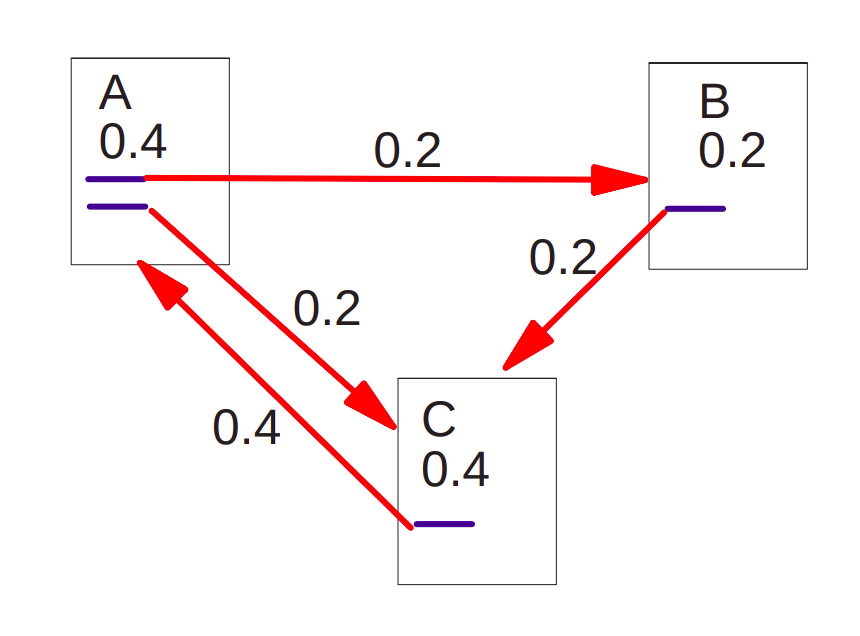
\includegraphics[scale=0.13]{webgraph.png}
				\end{figure}
				\column{0.6\textwidth}
				Power method solution:
				\begin{itemize}
					
				\vspace{0.2cm}
				\item Start with $ \vec{x}_0 = \mathtt{random()}$ \\
				\vspace{0.4cm}
				\item $\vec{x}_i = M \vec{x}_{i-1}$ \\
				\vspace{0.15cm}
				\hspace{0.5cm} until $ |\vec{x}_i -\vec{x}_{i-1}| < \epsilon$
				\end{itemize}
				
			\end{columns} 
		}

	
	
	\only<3>{
		
		Two problems:
		\vspace{0.2cm}
		\begin{itemize}
			\item \textbf{Dangling nodes}: pages without outgoing edges. How to assign probability to them?
			\vspace{0.3cm}
			\item \textbf{Pages without incoming or outgoing links} : node without incoming edges or group of nodes without outgoing edges. For the first ones we have probability 0 of returning to it once we leave it, while for the others we can never leave them once entered
		\end{itemize}	
		\vspace{0.2cm}
		
		}
		
		\only<4>{
			Allow the random surfer to move to a random page of the graph with probability $\alpha$.	\\
			\vspace{0.2cm}
			The stochastic matrix will be:
			\begin{eqnarray}
				\nonumber
				M' &=& (1-\alpha) M + \alpha \left[ \frac{1}{N} \right]_{N \times N} \\
				\nonumber
				&=& (1-\alpha) M + \alpha \vec{1}^T \cdot \vec{J}  
			\end{eqnarray}
		
		where $\vec{J} = (1/N, ... , 1/N)$ is the \textit{jump vector}
		}
	\end{frame}

	\begin{frame}[t]
		\frametitle{A recap of Topic-Sensitive PageRank}
		\framesubtitle{\textit{From Taher H. Haveliwala (2003)}}
		
		\onslide*<1->{ In addition to the PageRank calculation we can \textit{specialize} the scores of the pages by limiting them to a single topic. \\
		\vspace{0.3cm}
		For a given topic-specific set of pages $S$, we allow the random surfer to teleport only to pages that are inside $S$
		}
	
		\onslide*<2->{
		
			$$ M' = (1-\alpha) M + \alpha \vec{1}^T \cdot \vec{J_S}  $$
			
			where the \textit{topic-specific jump vector} is defined as 
			 
			\begin{equation}\nonumber
				J_{S_i}=\begin{cases}
					1/|S|, & \text{if page $i \in S$}.\\
					0, & \text{otherwise}.
				\end{cases}
			\end{equation}
			
				
					}
	\end{frame}
	
	
	\section{Wikipedia dataset}
	
	\begin{frame}
		\frametitle{Wikipedia ...}
		content...
	\end{frame}

	\section{WikipediaSearch implementation}
	
	\begin{frame}
		\frametitle{PageRank implementation}
	\end{frame}

	\section{WikipediaSearch evaluation}
	
	\begin{frame}
		\frametitle{Standard PageRank}
	\end{frame}
	
	\section{Conclusion}
		
	\begin{frame}
		\frametitle{Conclusion}
	\end{frame}
	
\end{document}